%\documentclass[conference, onecolumn]{IEEEtran}
\documentclass[11pt]{article}
\usepackage[a4paper,left=3cm,right=3cm,top=3cm,bottom=3.75cm,footskip=1.5cm,headsep=1cm]{geometry}

%\IEEEoverridecommandlockouts
% The preceding line is only needed to identify funding in the first footnote. If that is unneeded, please comment it out.
\usepackage{cite}
\usepackage{listings}
\usepackage{tikz}
\usepackage{amsmath,amssymb,amsfonts}
\usepackage{algorithmic}
\usepackage{graphicx}
\usepackage{textcomp}
\usepackage{xcolor}
\usepackage{url}

\renewcommand{\figurename}{Abbildung}

\def\BibTeX{{\rm B\kern-.05em{\sc i\kern-.025em b}\kern-.08em
    T\kern-.1667em\lower.7ex\hbox{E}\kern-.125emX}}

\newcommand\YAMLcolonstyle{\color{red}\mdseries}
\newcommand\YAMLkeystyle{\color{black}\bfseries}
\newcommand\YAMLvaluestyle{\color{blue}\mdseries}

\makeatletter

% here is a macro expanding to the name of the language
% (handy if you decide to change it further down the road)
\newcommand\language@yaml{yaml}

\expandafter\expandafter\expandafter\lstdefinelanguage
\expandafter{\language@yaml}
{
  keywords={true,false,null,y,n},
  keywordstyle=\color{darkgray}\bfseries,
  basicstyle=\YAMLkeystyle,                                 % assuming a key comes first
  sensitive=false,
  comment=[l]{\#},
  morecomment=[s]{/*}{*/},
  commentstyle=\color{purple}\ttfamily,
  stringstyle=\YAMLvaluestyle\ttfamily,
  moredelim=[l][\color{orange}]{\&},
  moredelim=[l][\color{magenta}]{*},
  moredelim=**[il][\YAMLcolonstyle{:}\YAMLvaluestyle]{:},   % switch to value style at :
  morestring=[b]',
  morestring=[b]",
  literate =    {---}{{\ProcessThreeDashes}}3
                {>}{{\textcolor{red}\textgreater}}1     
                {|}{{\textcolor{red}\textbar}}1 
                {\ -\ }{{\mdseries\ -\ }}3,
}

% switch to key style at EOL
\lst@AddToHook{EveryLine}{\ifx\lst@language\language@yaml\YAMLkeystyle\fi}
\makeatother

\newcommand\ProcessThreeDashes{\llap{\color{cyan}\mdseries-{-}-}}

\begin{document}

\title{Projektarbeit: Unmanned Surface Vehicle}

%\author{\IEEEauthorblockN{Josephine Brauer}
%\\
%\and
%\IEEEauthorblockN{Kilian Schweppe}
%\\
%}
\author{Josephine Brauer \and Kilian Schweppe}

\maketitle

\begin{abstract}
In dieser Projektarbeit wurde ein im Rahmen einer Bachelorarbeit entwickeltes Oberflächenfahrzeug für Wasserexploration in Rettungsszenarien durch Software ergänzt, die es ermöglicht, autonom ein Gewässer abzufahren und dabei die Wassertiefe zu erfassen.\\
Die notwendigen Funktionalitäten wurden in Python unter Nutzung von ROS und des von ROS bereitgestellten Navigation Stacks implementiert. Um die Funktionsweise testen zu können, wurde außerdem eine Simulation des Bootes auf Basis eines bestehenden Simulators erstellt.\\
Die richtige Funktionsweise des Bootes wurde im Simulator und auf der Wakenitz getestet.
\end{abstract}

\section{Einleitung}
Mit einem Anstieg der Anzahl der Naturkatastrophen und ihren verursachten Kosten in den letzten Jahrzehnten\cite{kellenberg} nimmt auch die Notwendigkeit zu, Möglichkeiten für die Verhinderung und Bewältigung von Katastrophen zu finden. Auch die Robotik bietet immer wieder Lösungen, die im Katastrophenschutz eingesetzt werden können. Dabei haben Unbemannte Fahrzeuge insbesondere zur Erfassung von Daten ein großes Potenzial \cite{surveyDisasterRobotics}.

Sie können Einsatzkräfte in unzugänglichen oder gefährlichen Umgebungen ersetzen \cite{bellingham}, welche damit sowohl geschützt, als auch anderen Aufgaben zugeteilt werden können. Durch die potenziell geringe Größe und Lautstärke der Fahrzeuge können auch Gebiete erfasst werden, die sonst entweder nicht zugänglich wären, oder unter größeren Eingriffen in die Natur leiden könnten, wie zum Beispiel Naturschutzgebiete. Mit unseren 201 Naturschutzgebieten in Schleswig-Holstein, und weiteren in Planung \cite{Naturschutz}, hat dieses Thema auch in unserer Region eine besondere Relevanz.

Besonders für lang andauernde Aufgaben und in Regionen, in denen man damit rechnen muss, nicht immer mit dem Fahrzeug kommunizieren zu können, kann es sinnvoll sein, diese Fahrzeuge nicht nur unbemannt, sondern auch autonom zu gestalten, da das Fahrzeug so nicht durchgehend angesteuert werden muss.

In Hinsicht auf Katastrophen spielt der Schutz vor Hochwasser in Schleswig-Holstein eine besondere Rolle, da laut der Landesregierung etwa ein Viertel der Landesfläche und mehr als 350.000 Menschen durch Sturmfluten gefährdet sind\cite{Hochwasser}. In Lübeck und Umgebung sind vor allem Flusshochwasser ein Problem (s. Abbildung \ref{Hochwassergefahrenkarte}). Hier könnten Unbemannte Wasserfahrzeuge zum Beispiel durch frühzeitiges Erkennen von Deichbrüchen helfen. Die denkbaren Anwendungsfelder sind allerdings nicht nur auf den Schutz vor Schäden durch unsere Gewässer begrenzt, vielmehr könnten sie auch den Schutz unserer Gewässer selbst abdecken, etwa durch Identifikation von Verschmutzungen und ihrer Quellen.

\begin{figure}
	\centering
	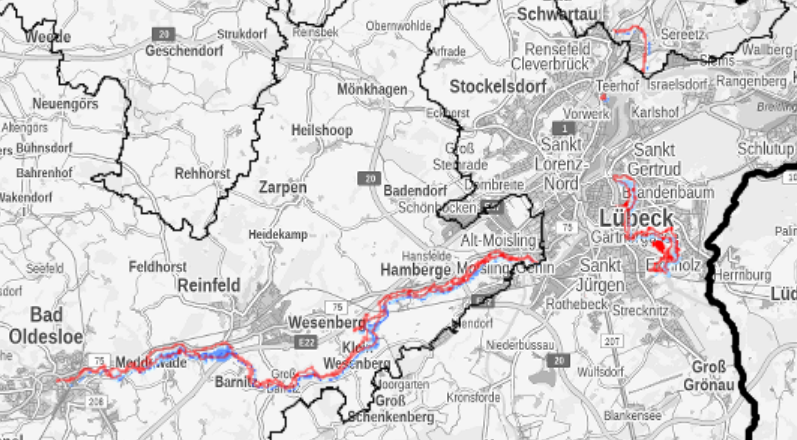
\includegraphics[width=0.8\linewidth]{Hochwasserrisiko.png}
	\caption{Hochwassergefahrenkarte für Hochwasser mit hoher Wahrscheinlichkeit, Quelle: \url{http://zebis.landsh.de/webauswertung/index.xhtml} ©GeoBasis-DE/LVermGeo SH, BKG}
	\label{Hochwassergefahrenkarte}
\end{figure}

Für den Einsatz im und auf dem Wasser sind unter anderem Unbemannte Unterwasserfahrzeuge (UUVs) und Unbemannte Oberflächenfahrzeuge (USVs) möglich \cite{surveyDisasterRobotics}. USVs haben dabei den Vorteil, mehr Sensoren über eine längere Zeitdauer tragen zu können und damit mehr verschiedene Messungen gleichzeitig über einen längeren Zeitraum durchführen zu können, wobei sowohl Messungen an der Oberfläche als auch im Wasser möglich sind \cite{coley2015}. Trotzdem wird ihnen bis jetzt in der Literatur weniger Beachtung gewidmet, als den Unbemannten Unterwasser Fahrzeugen \cite{surveyDisasterRobotics}.

Aus den genannten Gründen erscheint uns die Entwicklung autonomer USVs, die für vielfältige Szenarien im Bereich der Rettungsrobotik ausgerüstet sind, sinnvoll. In dieser Arbeit sollen dafür erste notwendige Schritte erfolgen, indem ein im Rahmen einer Bachelorarbeit entwickeltes Oberflächenfahrzeug für Wasserexploration in Rettungsszenarien durch Software ergänzt wird, die das autonome Befahren eines Gewässers ermöglicht. Des Weiteren wollen wir ein Anwendungsszenario, das Erfassen der Wassertiefe, implementieren und testen. Die Aufzeichnung der Wassertiefe könnte zum Beispiel hilfreich bei der Suche nach vermissten Personen oder Gegenständen, wie zum Beispiel Autos, sein.\\

Um die Funktionsweise des Bootes testen zu können, ohne Gefahr zu laufen, das Boot auf dem Wasser zu verlieren, und zukünftigen Gruppen die Arbeit mit dem Boot zu erleichtern, soll außerdem eine Simulation des Bootes auf Basis eines bestehenden Simulators erstellt werden.

\section{Methoden}
Da auf dem USV bereits ROS installiert und teilweise genutzt wird, liegt es nahe, vom von ROS bereitgestellten Navigation Stack \footnote{\url{https://github.com/ros-planning/navigation}} Gebrauch zu machen. Dieser bietet viele nützliche Funktionalitäten -unter anderem werden mehrere globale und lokale Planer bereitgestellt- für die autonome Navigation von mobilen Robotern \cite{zheng2019ros}. Es gibt sowohl ein Tutorial von ROS \footnote{\url{http://wiki.ros.org/navigation/Tutorials}}, als auch einige andere Quellen (z.B. \cite{zheng2019ros}), die sich mit der Benutzung des Navigation Stacks auseinandersetzen. Auf GitHub wurde das Projekt bis heute etwa 1400 Mal geforkt (Stand 08.03.2021). Das spricht für die Popularität des Navigation Stacks, weshalb angenommen werden kann, dass die Verwendung des Navigation Stacks die Verständlichkeit des Projekts auch für Außenstehende verbessert.

Auf Basis unserer Zielstellung haben wir mehrere Arbeitspakete identifiziert, auf deren Durchführung im Folgenden eingegangen werden soll:
\begin{enumerate}
	\item Auswahl des Simulators
	\item Einarbeitung in die Simulationsumgebung
	\item Simulation der Sensoren des Bootes
	\item Simulation der Ausgaben des Bootes
	\item Implementierung der Schnittstellen zum Navigation Stack
	\item Navigation zu Wegpunkten
	\item Vermeidung dynamischer Hindernisse
	\item Erstellung von Wegpunkten auf Basis der Karte
	\item Erfassung der Wassertiefe und Eintragung in Karte
	\item Schnittstellen zum Navigation Stack, Navigation zu Wegpunkten, Erstellung von Wegpunkten auf Basis der Karte und Erfassung der Wassertiefe auf das Boot übernehmen und -wenn notwendig- anpassen
\end{enumerate}

\subsection{Auswahl des Simulators}

Für die Suche eines geeigneten Simulators haben wir eine Literaturrecherche nach Webster und Watson \cite{webster2002} vorgenommen. Diese erfolgt nach der Auswahl der Stichworte und zu durchsuchender Datenbanken in drei Schritten:

\begin{enumerate}
	\item Durchsuchung der Datenbanken mit Hilfe der Stichworte nach relevanten Artikeln
	\item "Go backward" \cite{webster2002}: Betrachtung von Artikeln, die von den im ersten Schritt gefundenen Artikeln zitiert werden
	\item "Go forward" \cite{webster2002}: Betrachtung von Artikeln, in denen die im ersten Schritt gefundenen Artikel zitiert werden
\end{enumerate}

Als Stichworte haben wir folgende Begriffe gewählt:

\begin{itemize}
	\item Unmanned Surface Vehicle Simulation
	\item Unmanned Surface Vehicle Simulator
	\item Boat Simulation
	\item Boat Simulator
\end{itemize}

Wir haben als einzige Datenbank Google Scholar ausgewählt, da die meisten Archive wichtiger wissenschaftlicher Verlage in dieser Datenbank abgedeckt werden \cite{googlescholar}. Es wurden jeweils die ersten 10 Treffer nach passenden Simulatoren durchsucht. Nur für Paper, die einen relevanten verfügbaren Simulator benutzen, wurde eine Vorwärts- und Rückwärtssuche durchgeführt.\\

Wir haben uns entschieden, das USV im \textit{Unmanned Surface Vehicle Simulator with Realistic Environmental Disturbances} \footnote{\url{https://github.com/disaster-robotics-proalertas/usv_sim_lsa}} zu simulieren.

Der Master-Branch des Simulators benutzt ROS Kinetic. Da auf dem USV aber momentan ROS Melodic läuft und darüber hinaus Kinetic nach April 2021 nicht mehr von ROS unterstützt wird \cite{rosdistros}, hielten wir es für sinnvoll, zu versuchen, den Simulator auf ROS Melodic laufen zu lassen. Obwohl das Projekt über einen dafür vorgesehenen Branch \footnote{\url{https://github.com/disaster-robotics-proalertas/usv_sim_lsa/tree/master-melodic}} verfügt, mussten wir dieses Vorhaben letztendlich aus Zeitgründen und aufgrund von für uns nicht lokalisierbaren Problemen abbrechen und mit Kinetic weiterarbeiten.

\subsection{Einarbeitung in die Simulationsumgebung}

Da das Projekt nicht optimal dokumentiert ist, hat die Einarbeitung in den Simulator mehr Zeit in Anspruch genommen, als ursprünglich gedacht. Der Übersichtlichkeit halber wollen wir hier einen Überblick über die Bestandteile geben, die für unser Projekt angepasst wurden:\\
Die Simulationsumgebung stellt 4 verschiedene Boot-Modelle bereit: ein Airboot, ein Differentialboot, ein Ruderboot und ein Segelboot \cite{paravisi2019}. Wir haben das Differentialboot-Modell als Grundlage für unser Modell genommen, da es sich bei unserem USV ebenfalls um ein Boot mit 2 Motoren am Heck (s. Abbildung \ref{boot}) handelt. Wir haben 2 Dateien identifiziert, die das Boot modellieren: \texttt{diffboat.xacro}\footnote{\url{https://github.com/disaster-robotics-proalertas/usv_sim_lsa/blob/master/usv_sim/xacro/diffboat.xacro}} (modelliert unter anderem die Motoren) und \texttt{boat\_subdivided\_validated.xacro}\footnote{\url{https://github.com/disaster-robotics-proalertas/usv_sim_lsa/blob/master/usv_sim/xacro/boat_subdivided_validated.xacro}} (modelliert unter anderem Sensoren). Diese Dateien wurden als Grundlage genutzt, um unser Boot zu modellieren.

Die Szenarien befinden sich im Ordner \texttt{scenes}. Durch die Bearbeitung der XML-Dateien kann man z.B. die Anzahl und Positionen der Boote und Bojen, die Position und Art des Terrains und die Position der Kamera anpassen.\\
Ebenfalls hilfreich für die Erstellung neuer Szenarien sind die launch-Dateien in den folgenden Ordnern:

\begin{itemize}
	\item \texttt{usv\_sim\_lsa/usv\_sim/launch/scenarios\_launchs/}: hier kann man unter anderem die zu verwendende Welt angeben.
	\item \texttt{usv\_sim\_lsa/usv\_sim/launch/models/}: hier werden unter anderem die Nodes gestartet, die "auf dem Boot laufen", also zum Beispiel Nodes, die Transformationen publishen oder die Bewegungen des Bootes kontrollieren.
\end{itemize}

\subsection{Simulation der Sensoren des Bootes}

Auf dem Boot sind mehrere Sensoren zu finden:

\begin{itemize}
	\item ein GPS-Gerät
	\item ein Kompass
	\item ein Ultraschallsensor für die Wassertiefe
	\item ein Ultraschallsensor für die Erkennung von Hindernissen am Bug
	\item eine 360°-Kamera
	\item ein Temperatursensor
\end{itemize}

Darüber hinaus verfügt das Boot noch über 2 Motoren für die Fortbewegung und eine 4G/WIFI-Anbindung zur Kommunikation (s. Abbildung \ref{boot}).\\

\begin{figure}
    \centering
	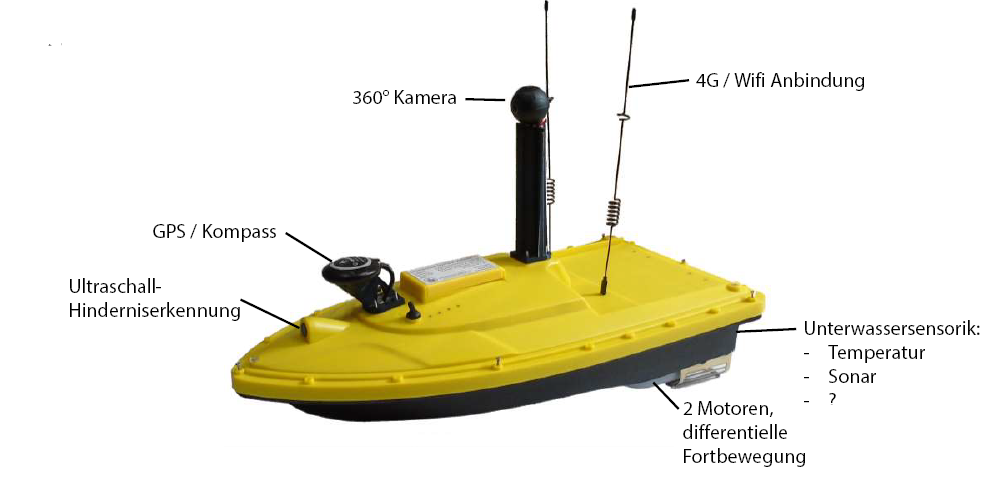
\includegraphics[width=0.9\linewidth]{boot.png}
	\caption{Sensoren und Aktuatoren des Bootes}
	\label{boot}
\end{figure}

Detaillierte Informationen zu allen Sensoren und Aktuatoren des Bootes und den erwarteten Ein- und Ausgabewerten lassen sich im zugehörigen GitHub-Projekt finden \footnote{\url{https://github.com/NRottmann/UzL_USV/}}.
Für die Implementierung unseres Szenarios in der Simulation benötigten wir die GPS-, Kompass- und Ultraschalldaten und die Motoren. Deshalb haben wir ein GPS-Modul und zwei Ultraschall-Sensoren zum Differentialboot-Modell des Simulators hinzugefügt. Außerdem haben wir das Modell durch eine IMU zur Simulierung der Orientierung ergänzt. Dazu haben wir die GazeboRosGps, GazeboRosImu und GazeboRosSonar Plugins aus dem Paket \texttt{hector\_gazebo\_plugins}  \footnote{\url{https://github.com/tu-darmstadt-ros-pkg/hector_gazebo}} verwendet.

%\begin{figure}
%	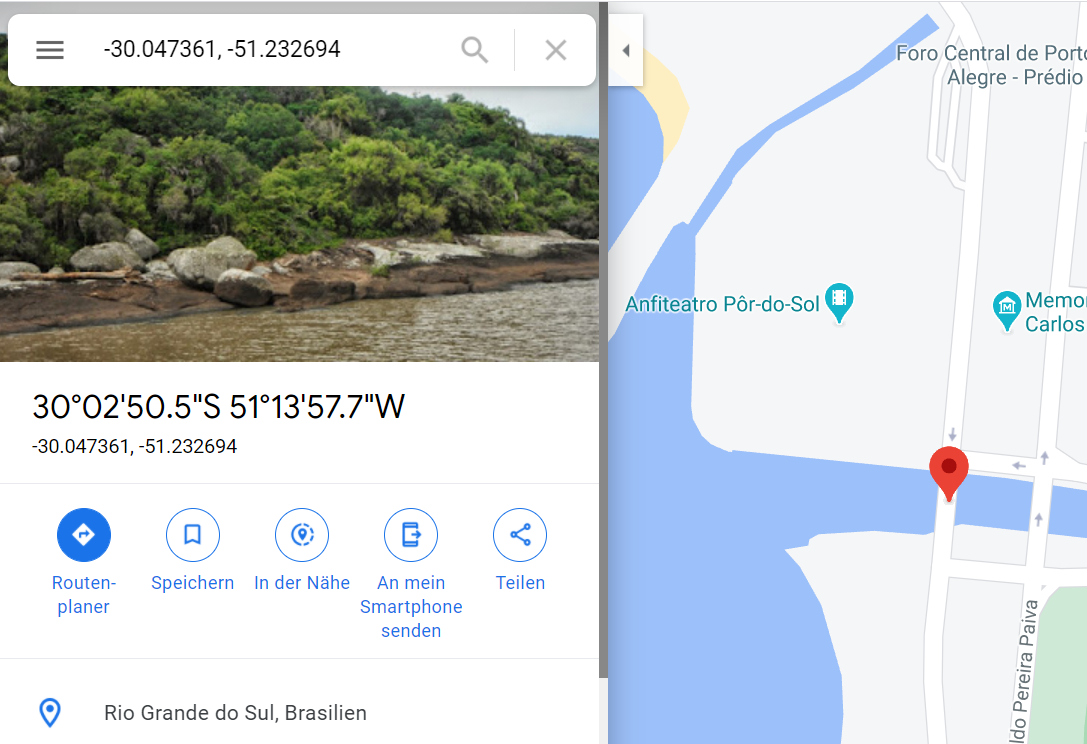
\includegraphics[width=\linewidth]{reference.png}
%	\caption{Referenzkoordinaten}
%	\label{reference}
%\end{figure}

Da wir für unser Szenario weitestgehend das \texttt{diffboat\_scenario1} übernommen haben (das einen Ausschnitt von Porto Alegre, Brasilien, nahe der Mündung des Dilúvio zeigt \cite{paravisi2019}), haben wir die GPS-Koordinaten eines markanten Punktes im Szenario bestimmt und als Referenzkoordinaten für die Simulierung der GPS-Daten gewählt.

\subsection{Simulation der Ausgaben des Bootes}

Nachdem wir die notwendigen Daten simuliert haben, die auch das echte Boot sammelt, wollten wir die Daten auch in derselben Form ausgeben, wie es das USV bereits tut. Dafür haben wir die notwendigen Topics und deren Inhalt bestimmt:

\begin{itemize}
	\item \texttt{range\_front}: Daten des vorderen Sonars
	\item \texttt{range\_depth}: Daten des unteren Sonars
	\item \texttt{velocity}: Geschwindigkeit des Bootes in Bewegungsrichtung
	\item \texttt{heading}: unterteilt sich in \texttt{gps\_heading}: die Bewegunsrichtung des Bootes und \texttt{mag\_heading}: die Orientierung des Bootes
	\item \texttt{gps}: GPS-Koordinaten des Bootes
	\item \texttt{safety}: Informationen zu Batteriestand, Spannung, Strom, Ladung und ob sich Wasser innerhalb des Bootes befindet
\end{itemize}
\texttt{range\_front}, \texttt{range\_depth} und \texttt{gps} konnten dabei als Parameter im jeweiligen XML-Element gegeben werden. Für das Publishen von \texttt{velocity} und \texttt{heading} haben wir die Simulationsumgebung durch Skripte ergänzt:
Die Geschwindigkeit des Bootes in Bewegungsrichtung, \texttt{velocity}, berechnen wir in \texttt{vel\_pub} über die Formel:

\begin{equation}
v = \sqrt{x^2+y^2}
\end{equation}

Dabei ist x die Geschwindigkeit in x-Richtung und y die Geschwindigkeit in y-Richtung.\\
Nach ROS-Konvention sollte die x-Achse Richtung Osten und die y-Achse Richtung Norden zeigen \cite{REP105}. An dieser Konvention haben wir uns bei der Implementierung orientiert. Wenn im Folgenden von x- oder y-Achse die Rede ist, sei damit auch immer die Achse in Richtung Osten oder Norden gemeint.\\
Deshalb können wir die beiden benötigten Werte aus dem Topic \texttt{gps/velocity} auslesen, welches vom simulierten GPS-Modul gepublisht wird.\\
Für \texttt{heading} bestimmen wir in \texttt{heading\_pub} die beiden Komponenten \texttt{gps\_heading} und \texttt{mag\_heading} einzeln:\\
Über 
\begin{equation}
	atan2(x,y) 	
\end{equation}
(wobei wieder x die Geschwindigkeit in x-Richtung und y die Geschwindigkeit in y-Richtung ist) bestimmen wir das \texttt{gps\_heading}, also die Bewegungsrichtung nach GPS. \\
Aus der Komponente \texttt{orientation} der simulierten IMU kann durch Umwandlung der ausgegebenen Quaternion in Euler-Winkel das \texttt{mag\_heading} bestimmt werden.\\
Beide Winkelangaben haben wir noch so angepasst, dass statt bei einer Orientierung Richtung Osten, bei einer Orientierung Richtung Norden 0° vorliegen. Beide Werte werden danach auf das Topic \texttt{heading} gepublisht. Einen Überblick der zur Simulierung der Ausgaben des Bootes genutzten Nodes findet sich in Abbildung \ref{output-sim-nodes}.\\

\begin{figure}
	\centering
	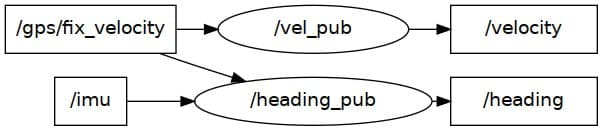
\includegraphics[width=0.7\linewidth]{simulation-nodes}
	\caption{Nodes zur Simulierung der Ausgaben des Bootes}
	\label{output-sim-nodes}
\end{figure}
Außerdem haben wir ein Skript \texttt{safety\_pub} hinzugefügt, dass den Batteriestand und den Wassersensor modelliert und aus das Topic \texttt{safety} publisht. Dabei wird ein linearer Abfall des Batteriestandes und eine Akkulaufzeit von 1h angenommen. Für den Wassersensor haben wir eine gewisse Wahrscheinlichkeit ausgewählt, mit der der Wert des Sensors auf 1 springt. Die Werte für Spannung, Strom und Ladung modellieren wir nicht, da sie für unser Szenario nicht relevant waren.
Außerdem haben wir auf das Publishen der folgenden Topics vorerst verzichtet, da diese für unseren Anwendungsfall nicht notwendig waren:
\begin{itemize}
	\item \texttt{mag}
	\item \texttt{temperature}
\end{itemize}

\subsection{Implementierung der Schnittstellen zum Navigation Stack}
Der Navigation Stack nutzt Odometrie- und Sensordaten, um Kommandos bezüglich der Geschwindigkeit an einen mobilen Roboter geben zu können, um einen bestimmte Zielkoordinaten zu erreichen. Damit dies möglich ist, müssen auf dem Roboter erst bestimmte Schnittstellen implementiert werden\cite{NavWiki}. In Abbildung \ref{nav} zu kann man mehrere Topics erkennen, die als Schnittstellen zwischen Roboter und Navigation Stack fungieren:
\begin{itemize}
	\item \texttt{odom}
	\item \texttt{map}
	\item \texttt{move\_base\_simple/goal}
	\item Sensor Topics des Formates LaserScan oder PointCloud
	\item \texttt{cmd\_vel}
\end{itemize}
Im Folgenden soll es darum gehen, wie wir die Werte der Topics generiert bzw. verarbeitet haben. Da wir in der Simulation dieselben Ausgabeschnittstellen erzeugt haben, wie wir sie auf dem echten Boot vorliegen haben werden, genügte in den meisten Fällen eine Implementierung der Schnittstellen zum Navigation Stack sowohl für die Simulation als auch für das echte Boot.

\begin{figure}
	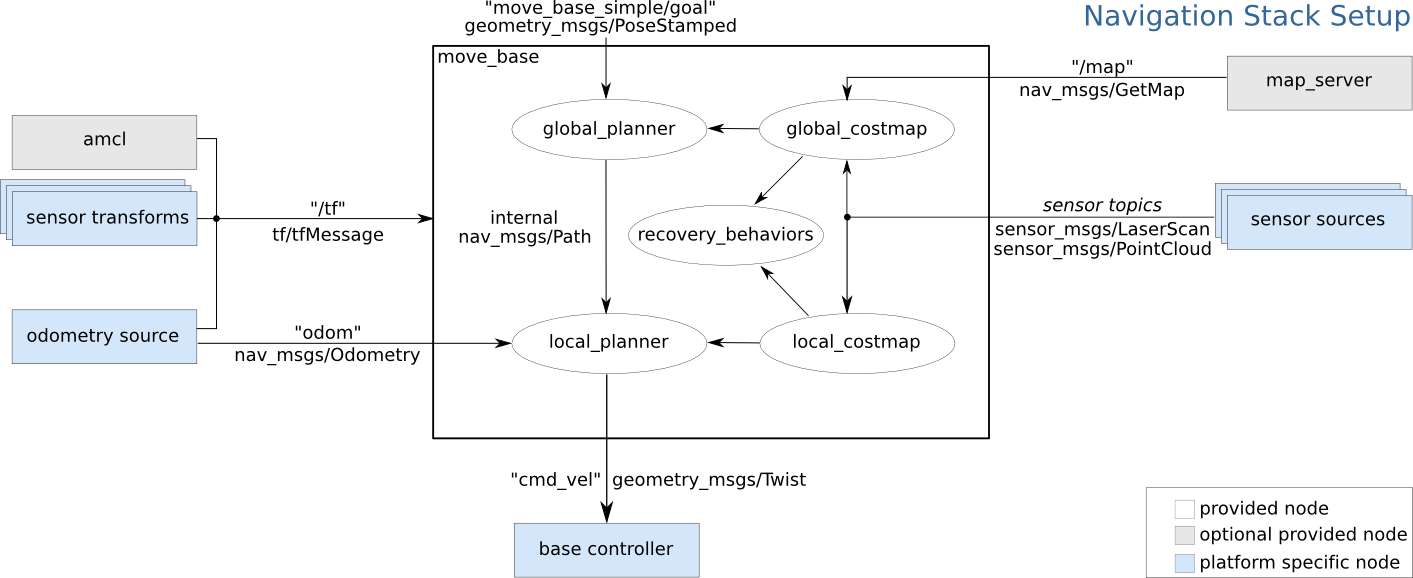
\includegraphics[width=\linewidth]{overview_tf.png}
	\caption{Robot Setup Navigation Stack (Quelle: http://wiki.ros.org/navigation/Tutorials/RobotSetup (Stand: 2018-07-19 02:43:42))}
	\label{nav}
\end{figure}

\subsubsection{odom}
Auf das Topic \texttt{/odom} schreiben wir die aktuellen Geschwindigkeiten des Bootes. Da wir die Frame ID des Bootes als \texttt{base\_link} festgelegt haben, sind die Position und Orientierung über die Position und Orientierung des \textit{frames} bekannt. Als Geschwindigkeit kann \texttt{velocity} übergeben werden.

\subsubsection{tf}

\begin{figure}
	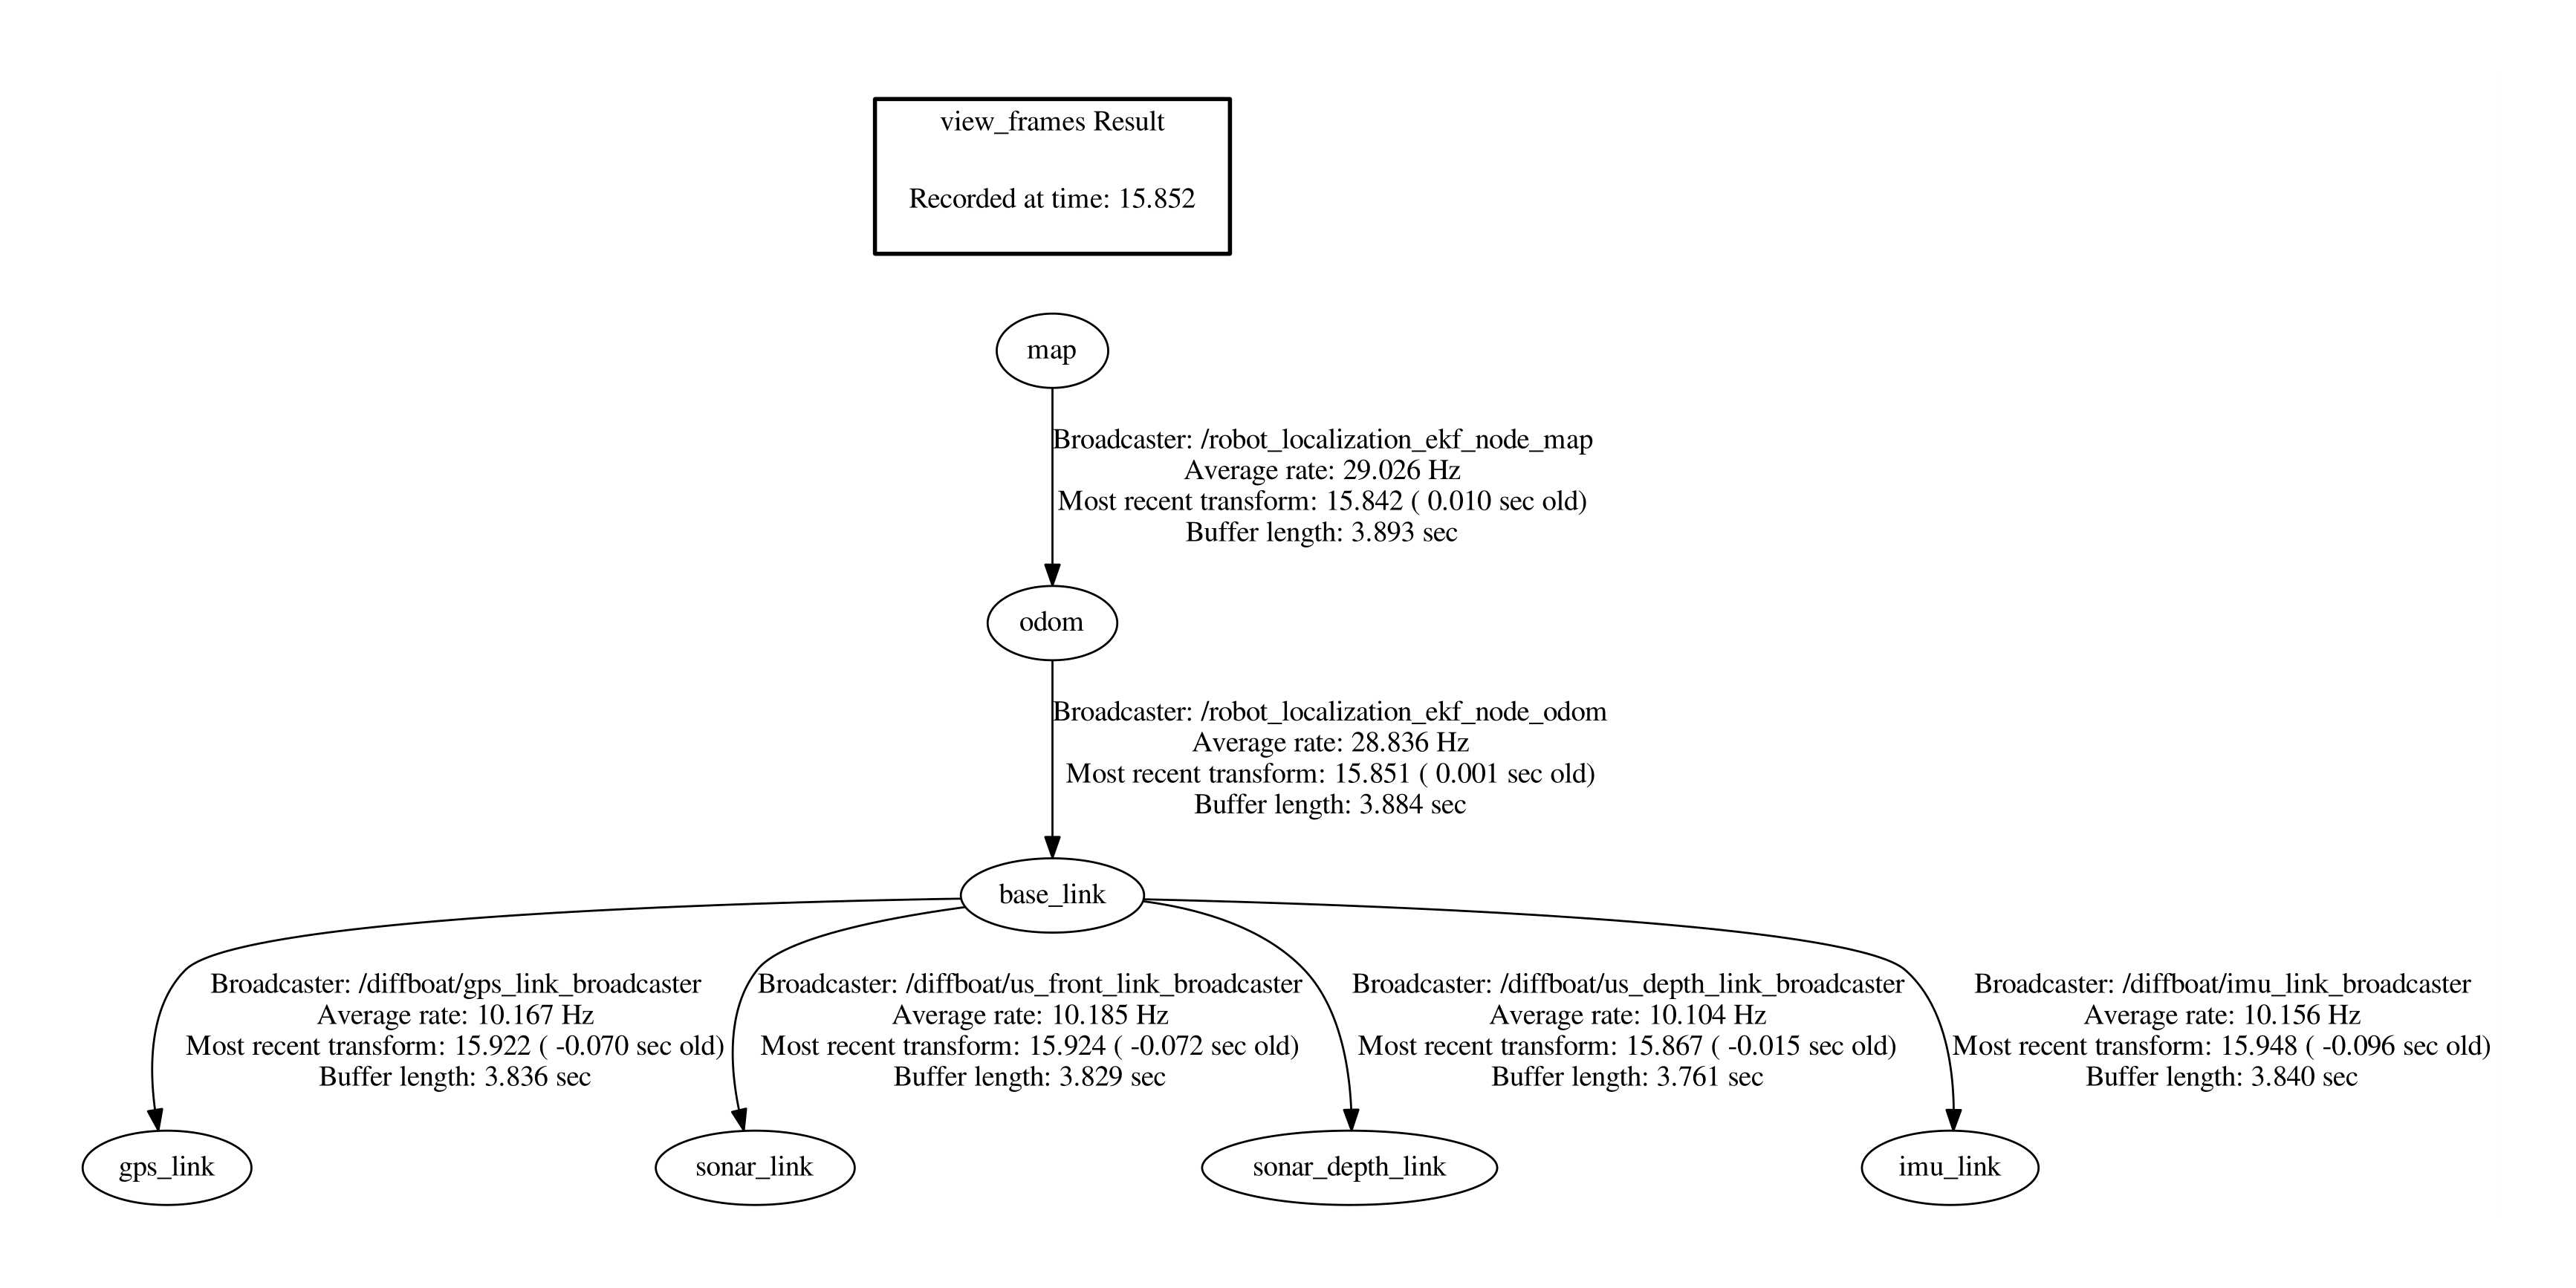
\includegraphics[width=\linewidth]{frames.png}
	\caption{Tf Tree}
	\label{frames}
\end{figure}

Der Navigation Stack benötigt 2 Transformationen um zu funktionieren, eine vom \texttt{map}-Frame zum \texttt{odom}-Frame und eine vom \texttt{odom}-Frame zum \texttt{base\_link}-Frame. Wie in \texttt{REP-105} \cite{REP105} spezifiziert, ist das \texttt{map}-Frame ein statisches Weltkoordinatensystem, welches die Position des Bootes in kartesischen Koordinaten auf der Karte darstellt.  Das \texttt{odom}-Frame ist ebenfalls ein statisches Koordinatensystem, in dem durch Auswertung der Odometrie die theoretische Position des Bootes bestimmt wird, welche zwar von der echten Position stark abweichen kann, aber dennoch eine genauere Lokalisierung ermöglicht.

Für die Erstellung dieser Transformationen setzen wir das \texttt{robot\_localization} \footnote{\url{http://wiki.ros.org/robot_localization}} Paket ein, welches die nötigen Transformationen bereits zur Verfügung stellt, GPS Koordinaten in Weltkoordinaten umrechnet und Sensorinformationen mit einem Kalman-Filter zusammenfügt \cite{MooreStouchKeneralizedEkf2014}. Den reultierenden Transformations-Tree einschließlich der statischen Transformationen ist in Abbildung \ref{frames} zu sehen.\\

Für die Transformation vom \texttt{odom}- zum \texttt{base\_link}-Frame nutzen wir den \texttt{ekf\_localization\_node}. Dieser kann Messages der Form:
\begin{itemize}
	\item Odom
	\item Imu
	\item Pose
	\item Twist
\end{itemize}
verwerten.
In unserem Fall wird die Geschwindigkeit in Bewegungsrichtung (\texttt{velocity}) für die Berechnung einer Odom-Message verwendet.
Außerdem benutzen wir \texttt{mag\_heading} und die aus der Ableitung von \texttt{mag\_heading} berechnete Winkelgeschwindigkeit zur Erzeugung einer IMU-Message.\\
Obwohl wir bei der Orientierung nach Kompass (\texttt{mag\_heading}) in Bewegung eine ungenauere Näherung an die Bewegungsrichtung erwarten, als die Orientierung nach GPS (\texttt{gps\_heading}) liefern würde, haben wir uns für die Verwendung von \texttt{mag\_heading} entschieden, da für die Berechnung der Odometrie kontinuierliche Daten erwartet werden \cite{REP105}. Bei \texttt{gps\_heading} kann es im Gegensatz zu \texttt{mag\_heading} zu diskreten Sprüngen kommen.\\

Für die Lokalisierung im Weltkoordinatensystem (also im \texttt{map}-Frame) wurde ebenfalls ein \texttt{ekf\_localization\_node} aufgesetzt. Dieser bekommt eine Odom-Message von einem \texttt{navsat\_transform\_node} \footnote{\url{http://docs.ros.org/en/noetic/api/robot_localization/html/navsat_transform_node.html}}, der die Daten vom Topic \texttt{gps} entsprechend umwandelt. Eine Übersicht der genutzten Nodes ist in Abbildung \ref{localization-overview} zu sehen.

\begin{figure}
	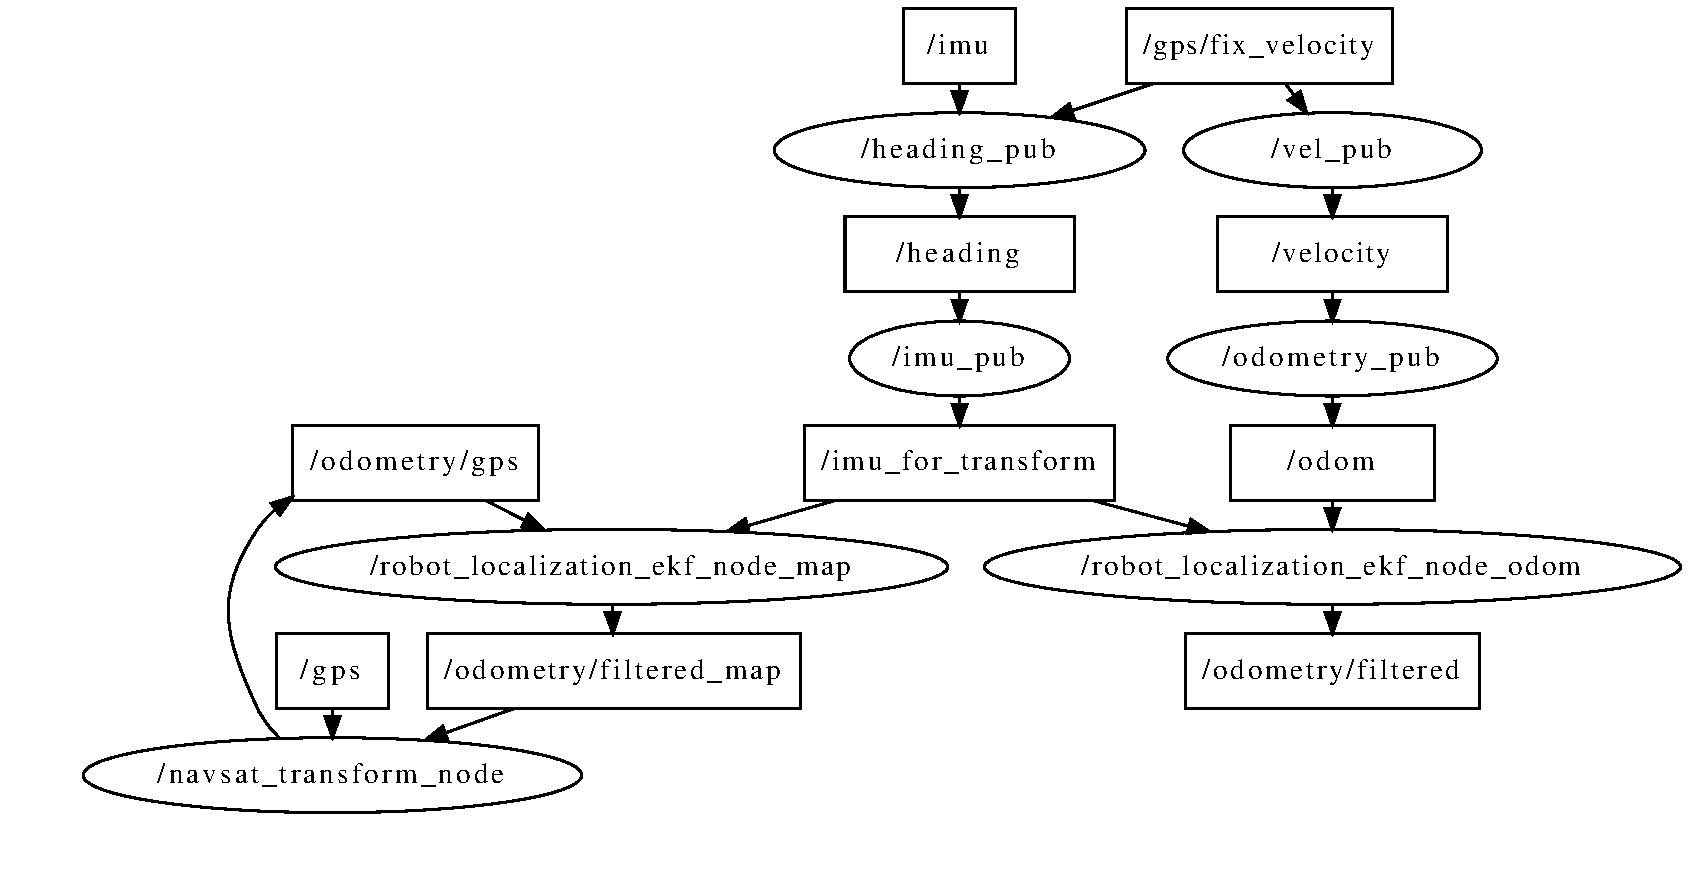
\includegraphics[width=\linewidth]{localization-nodes}
	\caption{Localization Nodes}
	\label{localization-overview}
\end{figure}

\subsubsection{map}

\begin{figure}
    \centering
	
\includegraphics[width=0.7\linewidth]{diluvio.jpg}
	\caption{Simulierte Region, © OpenStreetMap-Mitwirkende}
	\label{diluvio}
\end{figure}

Für den Map Server haben wir je eine schwarz-weiß Karte der in der Simulation dargestellten Region (\ref{diluvio}) und der Wakenitz mit Hilfe von OpenStreetMaps \footnote{\url{www.openstreetmap.org/copyright}} erstellt. Dabei stellen weiße Regionen befahrbare und schwarze unbefahrbare Gebiete dar.\\
Wichtige Informationen über die Karte, wie die Anzahl der Meter pro Pixel, sowie die Platzierung der linken unteren Ecke in der Simulationsumgebung haben wir berechnet und in einer yaml-Datei gespeichert.

\subsubsection{move\_base\_simple/goal} \label{goal}
Statt direkt auf das Topic \texttt{move\_base\_simple/goal} zu publishen, benutzen wir die \texttt{actionlib} API \footnote{\url{http://wiki.ros.org/actionlib}}. Diese hat den Vorteil, dass man direkt eine Callback-Methode übergeben kann, die aufgerufen wird, wenn das übergebene Ziel erreicht wurde. Das ist für uns besonders nützlich, da wir so die Messwerte an bestimmten Positionen leicht speichern können (s. \ref{measurements}).

\subsubsection{Sensor Topics}
Statt die normalerweise vom Navigation Stack genutzten \texttt{LaserScan}-Topics und \texttt{PointCloud}-Topics zu nutzen, um Hindernisse in die globale und lokale Costmap eintragen zu können und so auch unerwarteten Hindernissen ausweichen zu können, nutzen wir das \texttt{range\_sensor\_layer}-Plugin \footnote{\url{http://wiki.ros.org/range_sensor_layer}}, um die Daten des vorderen Ultraschallsensors direkt verwenden zu können. Im Vergleich zur Nutzung der Ultraschall-Daten zur Erstellung einer \texttt{PointCloud}-Message, lieferte diese Herangehensweise die besseren Resultate, da dabei dynamische Hindernisse in den Tests häufig nicht umfahren wurden.

\subsubsection{cmd\_vel} \label{cmd}
Die Werte aus \texttt{cmd\_vel} werden in Übereinstimmung mit den vom Boot erwarteten Werten in dem Skript \texttt{boat\_diff\_vel\_ctrl} in Werte zwischen -100 und 100 umgewandelt und dann auf die Motoren des Bootes geschrieben.

\subsection{Navigation zu Wegpunkten}

Die tatsächliche Navigation zu den Wegpunkten ist nach Implementierung der Schnittstellen Aufgabe des Navigation Stacks (durch das Publishen des Topics \texttt{cmd\_vel}).\\
In Testläufen mit reiner Verarbeitung der \texttt{cmd\_vel}-Werte konnte kein sicheres Anfahren der Zielpunkte erreicht werden, obwohl mehrere lokale Planer mit unterschiedlichen Parametern ausprobiert wurden. Der stabilste Planer schien der \texttt{teb\_local\_planner} \footnote{\url{http://wiki.ros.org/teb_local_planner}} zu sein, weshalb wir uns letztendlich für diesen entschieden haben. Die Parameter, die von den Standardeinstellungen abweichen, sind in Listing \ref{local-planner} zu sehen.\\
\lstinputlisting[label={local-planner}, caption={Parameter des lokalen Planers}, language=yaml]{../base_local_planner_params.yaml}
Wir vermuteten als Grund für die mäßige Leistung der lokalen Planer, dass das vom Navigation Stack geforderte Verhalten im Wasser später auftritt, als es an Land der Fall wäre und vom Navigation Stack erwartet wird. Daraufhin haben wir die Verarbeitung des Topics noch durch zwei PI-Regler ergänzt, indem wir den PI-Regler aus dem Skript \texttt{boat\_diff\_vel\_ctrl} des Simulators an unsere Gegebenheiten angepasst haben. Einer der Regler gleicht die lineare Geschwindigkeit an, der andere die Winkelgeschwindigkeit.

\subsection{Vermeidung dynamischer Hindernisse}


\subsection{Erstellung von Wegpunkten auf Basis der Karte}
Zur Erstellung der Wegpunkte müssen die GPS-Koordinaten der linken unteren Ecke eines abzufahrenden Bereichs angegeben werden, sowie die Höhe und Breite des abzufahrenden Bereichs in Metern. Außerdem kann ein Intervall in Metern angegeben werden, das den Abstand angibt, in dem Messwerte aufgenommen werden sollen. Um ein möglichst schnelles Abfahren des Bereichs zu gewährleisten, wird der nächste Zielpunkt des Bootes entlang der längeren Seite des Rechtecks gewählt, wenn möglich. Ist der Bereich durch ein Hindernis blockiert, wird einfach nach dem nächstmöglichen Zielpunkt nach demselben Prinzip gesucht. So wir ein Abfahren des gewünschten Bereichs in Zick-Zack-Linien erreicht (s. Abbildung \ref{Fahrtplanung}).

\begin{figure}
	\centering
	\resizebox{0.8\textwidth}{!}{\begin{pgfpicture}
\pgfpathrectangle{\pgfpointorigin}{\pgfqpoint{62.0000bp}{33.0000bp}}
\pgfusepath{use as bounding box}
\begin{pgfscope}
\definecolor{fc}{rgb}{0.5020,0.5020,0.5020}
\pgfsetfillcolor{fc}
\pgfsetfillopacity{0.4000}
\pgfsetlinewidth{0.5000bp}
\definecolor{sc}{rgb}{0.0000,0.0000,0.0000}
\pgfsetstrokecolor{sc}
\pgfsetmiterjoin
\pgfsetbuttcap
\pgfpathqmoveto{53.5000bp}{33.0000bp}
\pgfpathqcurveto{55.7091bp}{33.0000bp}{57.5000bp}{32.1046bp}{57.5000bp}{31.0000bp}
\pgfpathqcurveto{57.5000bp}{29.8954bp}{55.7091bp}{29.0000bp}{53.5000bp}{29.0000bp}
\pgfpathqcurveto{53.4030bp}{29.0000bp}{53.3068bp}{29.0017bp}{53.2116bp}{29.0051bp}
\pgfpathqcurveto{53.1748bp}{29.0017bp}{53.1376bp}{29.0000bp}{53.1000bp}{29.0000bp}
\pgfpathqcurveto{52.3000bp}{29.0000bp}{51.5000bp}{29.0000bp}{50.7000bp}{29.0000bp}
\pgfpathqcurveto{50.0373bp}{29.0000bp}{49.5000bp}{29.5373bp}{49.5000bp}{30.2000bp}
\pgfpathqcurveto{49.5000bp}{30.4667bp}{49.5000bp}{30.7333bp}{49.5000bp}{31.0000bp}
\pgfpathqcurveto{49.5000bp}{31.2667bp}{49.5000bp}{31.5333bp}{49.5000bp}{31.8000bp}
\pgfpathqcurveto{49.5000bp}{32.4627bp}{50.0373bp}{33.0000bp}{50.7000bp}{33.0000bp}
\pgfpathqcurveto{51.5000bp}{33.0000bp}{52.3000bp}{33.0000bp}{53.1000bp}{33.0000bp}
\pgfpathqcurveto{53.1376bp}{33.0000bp}{53.1748bp}{32.9983bp}{53.2116bp}{32.9949bp}
\pgfpathqcurveto{53.3068bp}{32.9983bp}{53.4030bp}{33.0000bp}{53.5000bp}{33.0000bp}
\pgfpathclose
\pgfusepathqfillstroke
\end{pgfscope}
\begin{pgfscope}
\definecolor{fc}{rgb}{0.5020,0.5020,0.5020}
\pgfsetfillcolor{fc}
\pgfsetfillopacity{0.4000}
\pgfsetlinewidth{0.5000bp}
\definecolor{sc}{rgb}{0.0000,0.0000,0.0000}
\pgfsetstrokecolor{sc}
\pgfsetmiterjoin
\pgfsetbuttcap
\pgfpathqmoveto{39.5000bp}{31.0000bp}
\pgfpathqcurveto{39.5000bp}{31.5523bp}{39.0523bp}{32.0000bp}{38.5000bp}{32.0000bp}
\pgfpathqcurveto{37.9477bp}{32.0000bp}{37.5000bp}{31.5523bp}{37.5000bp}{31.0000bp}
\pgfpathqcurveto{37.5000bp}{30.4477bp}{37.9477bp}{30.0000bp}{38.5000bp}{30.0000bp}
\pgfpathqcurveto{39.0523bp}{30.0000bp}{39.5000bp}{30.4477bp}{39.5000bp}{31.0000bp}
\pgfpathclose
\pgfusepathqfillstroke
\end{pgfscope}
\begin{pgfscope}
\definecolor{fc}{rgb}{0.5020,0.5020,0.5020}
\pgfsetfillcolor{fc}
\pgfsetfillopacity{0.4000}
\pgfsetlinewidth{0.5000bp}
\definecolor{sc}{rgb}{0.0000,0.0000,0.0000}
\pgfsetstrokecolor{sc}
\pgfsetmiterjoin
\pgfsetbuttcap
\pgfpathqmoveto{24.5000bp}{31.0000bp}
\pgfpathqcurveto{24.5000bp}{31.5523bp}{24.0523bp}{32.0000bp}{23.5000bp}{32.0000bp}
\pgfpathqcurveto{22.9477bp}{32.0000bp}{22.5000bp}{31.5523bp}{22.5000bp}{31.0000bp}
\pgfpathqcurveto{22.5000bp}{30.4477bp}{22.9477bp}{30.0000bp}{23.5000bp}{30.0000bp}
\pgfpathqcurveto{24.0523bp}{30.0000bp}{24.5000bp}{30.4477bp}{24.5000bp}{31.0000bp}
\pgfpathclose
\pgfusepathqfillstroke
\end{pgfscope}
\begin{pgfscope}
\definecolor{fc}{rgb}{0.5020,0.5020,0.5020}
\pgfsetfillcolor{fc}
\pgfsetfillopacity{0.4000}
\pgfsetlinewidth{0.5000bp}
\definecolor{sc}{rgb}{0.0000,0.0000,0.0000}
\pgfsetstrokecolor{sc}
\pgfsetmiterjoin
\pgfsetbuttcap
\pgfpathqmoveto{9.5000bp}{31.0000bp}
\pgfpathqcurveto{9.5000bp}{31.5523bp}{9.0523bp}{32.0000bp}{8.5000bp}{32.0000bp}
\pgfpathqcurveto{7.9477bp}{32.0000bp}{7.5000bp}{31.5523bp}{7.5000bp}{31.0000bp}
\pgfpathqcurveto{7.5000bp}{30.4477bp}{7.9477bp}{30.0000bp}{8.5000bp}{30.0000bp}
\pgfpathqcurveto{9.0523bp}{30.0000bp}{9.5000bp}{30.4477bp}{9.5000bp}{31.0000bp}
\pgfpathclose
\pgfusepathqfillstroke
\end{pgfscope}
\begin{pgfscope}
\definecolor{fc}{rgb}{0.5020,0.5020,0.5020}
\pgfsetfillcolor{fc}
\pgfsetfillopacity{0.4000}
\pgfsetlinewidth{0.5000bp}
\definecolor{sc}{rgb}{0.0000,0.0000,0.0000}
\pgfsetstrokecolor{sc}
\pgfsetmiterjoin
\pgfsetbuttcap
\pgfpathqmoveto{9.5000bp}{16.0000bp}
\pgfpathqcurveto{9.5000bp}{16.5523bp}{9.0523bp}{17.0000bp}{8.5000bp}{17.0000bp}
\pgfpathqcurveto{7.9477bp}{17.0000bp}{7.5000bp}{16.5523bp}{7.5000bp}{16.0000bp}
\pgfpathqcurveto{7.5000bp}{15.4477bp}{7.9477bp}{15.0000bp}{8.5000bp}{15.0000bp}
\pgfpathqcurveto{9.0523bp}{15.0000bp}{9.5000bp}{15.4477bp}{9.5000bp}{16.0000bp}
\pgfpathclose
\pgfusepathqfillstroke
\end{pgfscope}
\begin{pgfscope}
\definecolor{fc}{rgb}{0.5020,0.5020,0.5020}
\pgfsetfillcolor{fc}
\pgfsetfillopacity{0.4000}
\pgfsetlinewidth{0.5000bp}
\definecolor{sc}{rgb}{0.0000,0.0000,0.0000}
\pgfsetstrokecolor{sc}
\pgfsetmiterjoin
\pgfsetbuttcap
\pgfpathqmoveto{24.5000bp}{16.0000bp}
\pgfpathqcurveto{24.5000bp}{16.5523bp}{24.0523bp}{17.0000bp}{23.5000bp}{17.0000bp}
\pgfpathqcurveto{22.9477bp}{17.0000bp}{22.5000bp}{16.5523bp}{22.5000bp}{16.0000bp}
\pgfpathqcurveto{22.5000bp}{15.4477bp}{22.9477bp}{15.0000bp}{23.5000bp}{15.0000bp}
\pgfpathqcurveto{24.0523bp}{15.0000bp}{24.5000bp}{15.4477bp}{24.5000bp}{16.0000bp}
\pgfpathclose
\pgfusepathqfillstroke
\end{pgfscope}
\begin{pgfscope}
\definecolor{fc}{rgb}{0.5020,0.5020,0.5020}
\pgfsetfillcolor{fc}
\pgfsetfillopacity{0.4000}
\pgfsetlinewidth{0.5000bp}
\definecolor{sc}{rgb}{0.0000,0.0000,0.0000}
\pgfsetstrokecolor{sc}
\pgfsetmiterjoin
\pgfsetbuttcap
\pgfpathqmoveto{39.5000bp}{16.0000bp}
\pgfpathqcurveto{39.5000bp}{16.5523bp}{39.0523bp}{17.0000bp}{38.5000bp}{17.0000bp}
\pgfpathqcurveto{37.9477bp}{17.0000bp}{37.5000bp}{16.5523bp}{37.5000bp}{16.0000bp}
\pgfpathqcurveto{37.5000bp}{15.4477bp}{37.9477bp}{15.0000bp}{38.5000bp}{15.0000bp}
\pgfpathqcurveto{39.0523bp}{15.0000bp}{39.5000bp}{15.4477bp}{39.5000bp}{16.0000bp}
\pgfpathclose
\pgfusepathqfillstroke
\end{pgfscope}
\begin{pgfscope}
\definecolor{fc}{rgb}{0.5020,0.5020,0.5020}
\pgfsetfillcolor{fc}
\pgfsetfillopacity{0.4000}
\pgfsetlinewidth{0.5000bp}
\definecolor{sc}{rgb}{0.0000,0.0000,0.0000}
\pgfsetstrokecolor{sc}
\pgfsetmiterjoin
\pgfsetbuttcap
\pgfpathqmoveto{54.5000bp}{16.0000bp}
\pgfpathqcurveto{54.5000bp}{16.5523bp}{54.0523bp}{17.0000bp}{53.5000bp}{17.0000bp}
\pgfpathqcurveto{52.9477bp}{17.0000bp}{52.5000bp}{16.5523bp}{52.5000bp}{16.0000bp}
\pgfpathqcurveto{52.5000bp}{15.4477bp}{52.9477bp}{15.0000bp}{53.5000bp}{15.0000bp}
\pgfpathqcurveto{54.0523bp}{15.0000bp}{54.5000bp}{15.4477bp}{54.5000bp}{16.0000bp}
\pgfpathclose
\pgfusepathqfillstroke
\end{pgfscope}
\begin{pgfscope}
\definecolor{fc}{rgb}{0.5020,0.5020,0.5020}
\pgfsetfillcolor{fc}
\pgfsetfillopacity{0.4000}
\pgfsetlinewidth{0.5000bp}
\definecolor{sc}{rgb}{0.0000,0.0000,0.0000}
\pgfsetstrokecolor{sc}
\pgfsetmiterjoin
\pgfsetbuttcap
\pgfpathqmoveto{54.5000bp}{1.0000bp}
\pgfpathqcurveto{54.5000bp}{1.5523bp}{54.0523bp}{2.0000bp}{53.5000bp}{2.0000bp}
\pgfpathqcurveto{52.9477bp}{2.0000bp}{52.5000bp}{1.5523bp}{52.5000bp}{1.0000bp}
\pgfpathqcurveto{52.5000bp}{0.4477bp}{52.9477bp}{0.0000bp}{53.5000bp}{0.0000bp}
\pgfpathqcurveto{54.0523bp}{0.0000bp}{54.5000bp}{0.4477bp}{54.5000bp}{1.0000bp}
\pgfpathclose
\pgfusepathqfillstroke
\end{pgfscope}
\begin{pgfscope}
\definecolor{fc}{rgb}{0.5020,0.5020,0.5020}
\pgfsetfillcolor{fc}
\pgfsetfillopacity{0.4000}
\pgfsetlinewidth{0.5000bp}
\definecolor{sc}{rgb}{0.0000,0.0000,0.0000}
\pgfsetstrokecolor{sc}
\pgfsetmiterjoin
\pgfsetbuttcap
\pgfpathqmoveto{39.5000bp}{1.0000bp}
\pgfpathqcurveto{39.5000bp}{1.5523bp}{39.0523bp}{2.0000bp}{38.5000bp}{2.0000bp}
\pgfpathqcurveto{37.9477bp}{2.0000bp}{37.5000bp}{1.5523bp}{37.5000bp}{1.0000bp}
\pgfpathqcurveto{37.5000bp}{0.4477bp}{37.9477bp}{0.0000bp}{38.5000bp}{0.0000bp}
\pgfpathqcurveto{39.0523bp}{0.0000bp}{39.5000bp}{0.4477bp}{39.5000bp}{1.0000bp}
\pgfpathclose
\pgfusepathqfillstroke
\end{pgfscope}
\begin{pgfscope}
\definecolor{fc}{rgb}{0.5020,0.5020,0.5020}
\pgfsetfillcolor{fc}
\pgfsetfillopacity{0.4000}
\pgfsetlinewidth{0.5000bp}
\definecolor{sc}{rgb}{0.0000,0.0000,0.0000}
\pgfsetstrokecolor{sc}
\pgfsetmiterjoin
\pgfsetbuttcap
\pgfpathqmoveto{24.5000bp}{1.0000bp}
\pgfpathqcurveto{24.5000bp}{1.5523bp}{24.0523bp}{2.0000bp}{23.5000bp}{2.0000bp}
\pgfpathqcurveto{22.9477bp}{2.0000bp}{22.5000bp}{1.5523bp}{22.5000bp}{1.0000bp}
\pgfpathqcurveto{22.5000bp}{0.4477bp}{22.9477bp}{0.0000bp}{23.5000bp}{0.0000bp}
\pgfpathqcurveto{24.0523bp}{0.0000bp}{24.5000bp}{0.4477bp}{24.5000bp}{1.0000bp}
\pgfpathclose
\pgfusepathqfillstroke
\end{pgfscope}
\begin{pgfscope}
\definecolor{fc}{rgb}{0.5020,0.5020,0.5020}
\pgfsetfillcolor{fc}
\pgfsetfillopacity{0.4000}
\pgfsetlinewidth{0.5000bp}
\definecolor{sc}{rgb}{0.0000,0.0000,0.0000}
\pgfsetstrokecolor{sc}
\pgfsetmiterjoin
\pgfsetbuttcap
\pgfpathqmoveto{9.5000bp}{1.0000bp}
\pgfpathqcurveto{9.5000bp}{1.5523bp}{9.0523bp}{2.0000bp}{8.5000bp}{2.0000bp}
\pgfpathqcurveto{7.9477bp}{2.0000bp}{7.5000bp}{1.5523bp}{7.5000bp}{1.0000bp}
\pgfpathqcurveto{7.5000bp}{0.4477bp}{7.9477bp}{0.0000bp}{8.5000bp}{0.0000bp}
\pgfpathqcurveto{9.0523bp}{0.0000bp}{9.5000bp}{0.4477bp}{9.5000bp}{1.0000bp}
\pgfpathclose
\pgfusepathqfillstroke
\end{pgfscope}
\begin{pgfscope}
\pgfsetlinewidth{0.5000bp}
\definecolor{sc}{rgb}{0.0000,0.0000,0.0000}
\pgfsetstrokecolor{sc}
\pgfsetmiterjoin
\pgfsetbuttcap
\pgfpathqmoveto{7.5000bp}{16.0000bp}
\pgfpathqcurveto{3.4069bp}{15.5522bp}{-0.2743bp}{18.5073bp}{-0.7222bp}{22.6004bp}
\pgfpathqcurveto{-1.1700bp}{26.6935bp}{1.7851bp}{30.3747bp}{5.8782bp}{30.8226bp}
\pgfusepathqstroke
\end{pgfscope}
\begin{pgfscope}
\definecolor{fc}{rgb}{0.0000,0.0000,0.0000}
\pgfsetfillcolor{fc}
\pgfusepathqfill
\end{pgfscope}
\begin{pgfscope}
\definecolor{fc}{rgb}{0.0000,0.0000,0.0000}
\pgfsetfillcolor{fc}
\pgfusepathqfill
\end{pgfscope}
\begin{pgfscope}
\definecolor{fc}{rgb}{0.0000,0.0000,0.0000}
\pgfsetfillcolor{fc}
\pgfpathqmoveto{7.5000bp}{31.0000bp}
\pgfpathqlineto{5.6378bp}{31.3875bp}
\pgfpathqlineto{6.0089bp}{30.8369bp}
\pgfpathqlineto{5.7656bp}{30.2189bp}
\pgfpathqlineto{7.5000bp}{31.0000bp}
\pgfpathclose
\pgfusepathqfill
\end{pgfscope}
\begin{pgfscope}
\definecolor{fc}{rgb}{0.0000,0.0000,0.0000}
\pgfsetfillcolor{fc}
\pgfpathqmoveto{6.0089bp}{30.8369bp}
\pgfpathqlineto{5.8782bp}{30.8226bp}
\pgfpathqlineto{5.8511bp}{31.0711bp}
\pgfpathqlineto{6.0089bp}{30.8369bp}
\pgfpathqlineto{5.8782bp}{30.8226bp}
\pgfpathqlineto{5.9054bp}{30.5740bp}
\pgfpathqlineto{6.0089bp}{30.8369bp}
\pgfpathclose
\pgfusepathqfill
\end{pgfscope}
\begin{pgfscope}
\pgfsetlinewidth{0.5000bp}
\definecolor{sc}{rgb}{0.0000,0.0000,0.0000}
\pgfsetstrokecolor{sc}
\pgfsetmiterjoin
\pgfsetbuttcap
\pgfpathqmoveto{54.5000bp}{1.0000bp}
\pgfpathqcurveto{58.5931bp}{0.5522bp}{62.2743bp}{3.5073bp}{62.7222bp}{7.6004bp}
\pgfpathqcurveto{63.1700bp}{11.6935bp}{60.2149bp}{15.3747bp}{56.1218bp}{15.8226bp}
\pgfusepathqstroke
\end{pgfscope}
\begin{pgfscope}
\definecolor{fc}{rgb}{0.0000,0.0000,0.0000}
\pgfsetfillcolor{fc}
\pgfusepathqfill
\end{pgfscope}
\begin{pgfscope}
\definecolor{fc}{rgb}{0.0000,0.0000,0.0000}
\pgfsetfillcolor{fc}
\pgfusepathqfill
\end{pgfscope}
\begin{pgfscope}
\definecolor{fc}{rgb}{0.0000,0.0000,0.0000}
\pgfsetfillcolor{fc}
\pgfpathqmoveto{54.5000bp}{16.0000bp}
\pgfpathqlineto{56.2344bp}{15.2189bp}
\pgfpathqlineto{55.9911bp}{15.8369bp}
\pgfpathqlineto{56.3622bp}{16.3875bp}
\pgfpathqlineto{54.5000bp}{16.0000bp}
\pgfpathclose
\pgfusepathqfill
\end{pgfscope}
\begin{pgfscope}
\definecolor{fc}{rgb}{0.0000,0.0000,0.0000}
\pgfsetfillcolor{fc}
\pgfpathqmoveto{55.9911bp}{15.8369bp}
\pgfpathqlineto{56.1218bp}{15.8226bp}
\pgfpathqlineto{56.0946bp}{15.5740bp}
\pgfpathqlineto{55.9911bp}{15.8369bp}
\pgfpathqlineto{56.1218bp}{15.8226bp}
\pgfpathqlineto{56.1489bp}{16.0711bp}
\pgfpathqlineto{55.9911bp}{15.8369bp}
\pgfpathclose
\pgfusepathqfill
\end{pgfscope}
\begin{pgfscope}
\pgfsetlinewidth{0.5000bp}
\definecolor{sc}{rgb}{0.0000,0.0000,0.0000}
\pgfsetstrokecolor{sc}
\pgfsetmiterjoin
\pgfsetbuttcap
\pgfpathqmoveto{39.5000bp}{31.0000bp}
\pgfpathqlineto{47.8686bp}{31.0000bp}
\pgfusepathqstroke
\end{pgfscope}
\begin{pgfscope}
\definecolor{fc}{rgb}{0.0000,0.0000,0.0000}
\pgfsetfillcolor{fc}
\pgfusepathqfill
\end{pgfscope}
\begin{pgfscope}
\definecolor{fc}{rgb}{0.0000,0.0000,0.0000}
\pgfsetfillcolor{fc}
\pgfusepathqfill
\end{pgfscope}
\begin{pgfscope}
\definecolor{fc}{rgb}{0.0000,0.0000,0.0000}
\pgfsetfillcolor{fc}
\pgfpathqmoveto{49.5000bp}{31.0000bp}
\pgfpathqlineto{47.6910bp}{31.5878bp}
\pgfpathqlineto{48.0000bp}{31.0000bp}
\pgfpathqlineto{47.6910bp}{30.4122bp}
\pgfpathqlineto{49.5000bp}{31.0000bp}
\pgfpathclose
\pgfusepathqfill
\end{pgfscope}
\begin{pgfscope}
\definecolor{fc}{rgb}{0.0000,0.0000,0.0000}
\pgfsetfillcolor{fc}
\pgfpathqmoveto{48.0000bp}{31.0000bp}
\pgfpathqlineto{47.8686bp}{31.0000bp}
\pgfpathqlineto{47.8686bp}{31.2500bp}
\pgfpathqlineto{48.0000bp}{31.0000bp}
\pgfpathqlineto{47.8686bp}{31.0000bp}
\pgfpathqlineto{47.8686bp}{30.7500bp}
\pgfpathqlineto{48.0000bp}{31.0000bp}
\pgfpathclose
\pgfusepathqfill
\end{pgfscope}
\begin{pgfscope}
\pgfsetlinewidth{0.5000bp}
\definecolor{sc}{rgb}{0.0000,0.0000,0.0000}
\pgfsetstrokecolor{sc}
\pgfsetmiterjoin
\pgfsetbuttcap
\pgfpathqmoveto{24.5000bp}{31.0000bp}
\pgfpathqlineto{35.8686bp}{31.0000bp}
\pgfusepathqstroke
\end{pgfscope}
\begin{pgfscope}
\definecolor{fc}{rgb}{0.0000,0.0000,0.0000}
\pgfsetfillcolor{fc}
\pgfusepathqfill
\end{pgfscope}
\begin{pgfscope}
\definecolor{fc}{rgb}{0.0000,0.0000,0.0000}
\pgfsetfillcolor{fc}
\pgfusepathqfill
\end{pgfscope}
\begin{pgfscope}
\definecolor{fc}{rgb}{0.0000,0.0000,0.0000}
\pgfsetfillcolor{fc}
\pgfpathqmoveto{37.5000bp}{31.0000bp}
\pgfpathqlineto{35.6910bp}{31.5878bp}
\pgfpathqlineto{36.0000bp}{31.0000bp}
\pgfpathqlineto{35.6910bp}{30.4122bp}
\pgfpathqlineto{37.5000bp}{31.0000bp}
\pgfpathclose
\pgfusepathqfill
\end{pgfscope}
\begin{pgfscope}
\definecolor{fc}{rgb}{0.0000,0.0000,0.0000}
\pgfsetfillcolor{fc}
\pgfpathqmoveto{36.0000bp}{31.0000bp}
\pgfpathqlineto{35.8686bp}{31.0000bp}
\pgfpathqlineto{35.8686bp}{31.2500bp}
\pgfpathqlineto{36.0000bp}{31.0000bp}
\pgfpathqlineto{35.8686bp}{31.0000bp}
\pgfpathqlineto{35.8686bp}{30.7500bp}
\pgfpathqlineto{36.0000bp}{31.0000bp}
\pgfpathclose
\pgfusepathqfill
\end{pgfscope}
\begin{pgfscope}
\pgfsetlinewidth{0.5000bp}
\definecolor{sc}{rgb}{0.0000,0.0000,0.0000}
\pgfsetstrokecolor{sc}
\pgfsetmiterjoin
\pgfsetbuttcap
\pgfpathqmoveto{9.5000bp}{31.0000bp}
\pgfpathqlineto{20.8686bp}{31.0000bp}
\pgfusepathqstroke
\end{pgfscope}
\begin{pgfscope}
\definecolor{fc}{rgb}{0.0000,0.0000,0.0000}
\pgfsetfillcolor{fc}
\pgfusepathqfill
\end{pgfscope}
\begin{pgfscope}
\definecolor{fc}{rgb}{0.0000,0.0000,0.0000}
\pgfsetfillcolor{fc}
\pgfusepathqfill
\end{pgfscope}
\begin{pgfscope}
\definecolor{fc}{rgb}{0.0000,0.0000,0.0000}
\pgfsetfillcolor{fc}
\pgfpathqmoveto{22.5000bp}{31.0000bp}
\pgfpathqlineto{20.6910bp}{31.5878bp}
\pgfpathqlineto{21.0000bp}{31.0000bp}
\pgfpathqlineto{20.6910bp}{30.4122bp}
\pgfpathqlineto{22.5000bp}{31.0000bp}
\pgfpathclose
\pgfusepathqfill
\end{pgfscope}
\begin{pgfscope}
\definecolor{fc}{rgb}{0.0000,0.0000,0.0000}
\pgfsetfillcolor{fc}
\pgfpathqmoveto{21.0000bp}{31.0000bp}
\pgfpathqlineto{20.8686bp}{31.0000bp}
\pgfpathqlineto{20.8686bp}{31.2500bp}
\pgfpathqlineto{21.0000bp}{31.0000bp}
\pgfpathqlineto{20.8686bp}{31.0000bp}
\pgfpathqlineto{20.8686bp}{30.7500bp}
\pgfpathqlineto{21.0000bp}{31.0000bp}
\pgfpathclose
\pgfusepathqfill
\end{pgfscope}
\begin{pgfscope}
\pgfsetlinewidth{0.5000bp}
\definecolor{sc}{rgb}{0.0000,0.0000,0.0000}
\pgfsetstrokecolor{sc}
\pgfsetmiterjoin
\pgfsetbuttcap
\pgfpathqmoveto{22.5000bp}{16.0000bp}
\pgfpathqlineto{11.1314bp}{16.0000bp}
\pgfusepathqstroke
\end{pgfscope}
\begin{pgfscope}
\definecolor{fc}{rgb}{0.0000,0.0000,0.0000}
\pgfsetfillcolor{fc}
\pgfusepathqfill
\end{pgfscope}
\begin{pgfscope}
\definecolor{fc}{rgb}{0.0000,0.0000,0.0000}
\pgfsetfillcolor{fc}
\pgfusepathqfill
\end{pgfscope}
\begin{pgfscope}
\definecolor{fc}{rgb}{0.0000,0.0000,0.0000}
\pgfsetfillcolor{fc}
\pgfpathqmoveto{9.5000bp}{16.0000bp}
\pgfpathqlineto{11.3090bp}{15.4122bp}
\pgfpathqlineto{11.0000bp}{16.0000bp}
\pgfpathqlineto{11.3090bp}{16.5878bp}
\pgfpathqlineto{9.5000bp}{16.0000bp}
\pgfpathclose
\pgfusepathqfill
\end{pgfscope}
\begin{pgfscope}
\definecolor{fc}{rgb}{0.0000,0.0000,0.0000}
\pgfsetfillcolor{fc}
\pgfpathqmoveto{11.0000bp}{16.0000bp}
\pgfpathqlineto{11.1314bp}{16.0000bp}
\pgfpathqlineto{11.1314bp}{15.7500bp}
\pgfpathqlineto{11.0000bp}{16.0000bp}
\pgfpathqlineto{11.1314bp}{16.0000bp}
\pgfpathqlineto{11.1314bp}{16.2500bp}
\pgfpathqlineto{11.0000bp}{16.0000bp}
\pgfpathclose
\pgfusepathqfill
\end{pgfscope}
\begin{pgfscope}
\pgfsetlinewidth{0.5000bp}
\definecolor{sc}{rgb}{0.0000,0.0000,0.0000}
\pgfsetstrokecolor{sc}
\pgfsetmiterjoin
\pgfsetbuttcap
\pgfpathqmoveto{37.5000bp}{16.0000bp}
\pgfpathqlineto{26.1314bp}{16.0000bp}
\pgfusepathqstroke
\end{pgfscope}
\begin{pgfscope}
\definecolor{fc}{rgb}{0.0000,0.0000,0.0000}
\pgfsetfillcolor{fc}
\pgfusepathqfill
\end{pgfscope}
\begin{pgfscope}
\definecolor{fc}{rgb}{0.0000,0.0000,0.0000}
\pgfsetfillcolor{fc}
\pgfusepathqfill
\end{pgfscope}
\begin{pgfscope}
\definecolor{fc}{rgb}{0.0000,0.0000,0.0000}
\pgfsetfillcolor{fc}
\pgfpathqmoveto{24.5000bp}{16.0000bp}
\pgfpathqlineto{26.3090bp}{15.4122bp}
\pgfpathqlineto{26.0000bp}{16.0000bp}
\pgfpathqlineto{26.3090bp}{16.5878bp}
\pgfpathqlineto{24.5000bp}{16.0000bp}
\pgfpathclose
\pgfusepathqfill
\end{pgfscope}
\begin{pgfscope}
\definecolor{fc}{rgb}{0.0000,0.0000,0.0000}
\pgfsetfillcolor{fc}
\pgfpathqmoveto{26.0000bp}{16.0000bp}
\pgfpathqlineto{26.1314bp}{16.0000bp}
\pgfpathqlineto{26.1314bp}{15.7500bp}
\pgfpathqlineto{26.0000bp}{16.0000bp}
\pgfpathqlineto{26.1314bp}{16.0000bp}
\pgfpathqlineto{26.1314bp}{16.2500bp}
\pgfpathqlineto{26.0000bp}{16.0000bp}
\pgfpathclose
\pgfusepathqfill
\end{pgfscope}
\begin{pgfscope}
\pgfsetlinewidth{0.5000bp}
\definecolor{sc}{rgb}{0.0000,0.0000,0.0000}
\pgfsetstrokecolor{sc}
\pgfsetmiterjoin
\pgfsetbuttcap
\pgfpathqmoveto{52.5000bp}{16.0000bp}
\pgfpathqlineto{41.1314bp}{16.0000bp}
\pgfusepathqstroke
\end{pgfscope}
\begin{pgfscope}
\definecolor{fc}{rgb}{0.0000,0.0000,0.0000}
\pgfsetfillcolor{fc}
\pgfusepathqfill
\end{pgfscope}
\begin{pgfscope}
\definecolor{fc}{rgb}{0.0000,0.0000,0.0000}
\pgfsetfillcolor{fc}
\pgfusepathqfill
\end{pgfscope}
\begin{pgfscope}
\definecolor{fc}{rgb}{0.0000,0.0000,0.0000}
\pgfsetfillcolor{fc}
\pgfpathqmoveto{39.5000bp}{16.0000bp}
\pgfpathqlineto{41.3090bp}{15.4122bp}
\pgfpathqlineto{41.0000bp}{16.0000bp}
\pgfpathqlineto{41.3090bp}{16.5878bp}
\pgfpathqlineto{39.5000bp}{16.0000bp}
\pgfpathclose
\pgfusepathqfill
\end{pgfscope}
\begin{pgfscope}
\definecolor{fc}{rgb}{0.0000,0.0000,0.0000}
\pgfsetfillcolor{fc}
\pgfpathqmoveto{41.0000bp}{16.0000bp}
\pgfpathqlineto{41.1314bp}{16.0000bp}
\pgfpathqlineto{41.1314bp}{15.7500bp}
\pgfpathqlineto{41.0000bp}{16.0000bp}
\pgfpathqlineto{41.1314bp}{16.0000bp}
\pgfpathqlineto{41.1314bp}{16.2500bp}
\pgfpathqlineto{41.0000bp}{16.0000bp}
\pgfpathclose
\pgfusepathqfill
\end{pgfscope}
\begin{pgfscope}
\pgfsetlinewidth{0.5000bp}
\definecolor{sc}{rgb}{0.0000,0.0000,0.0000}
\pgfsetstrokecolor{sc}
\pgfsetmiterjoin
\pgfsetbuttcap
\pgfpathqmoveto{39.5000bp}{1.0000bp}
\pgfpathqlineto{50.8686bp}{1.0000bp}
\pgfusepathqstroke
\end{pgfscope}
\begin{pgfscope}
\definecolor{fc}{rgb}{0.0000,0.0000,0.0000}
\pgfsetfillcolor{fc}
\pgfusepathqfill
\end{pgfscope}
\begin{pgfscope}
\definecolor{fc}{rgb}{0.0000,0.0000,0.0000}
\pgfsetfillcolor{fc}
\pgfusepathqfill
\end{pgfscope}
\begin{pgfscope}
\definecolor{fc}{rgb}{0.0000,0.0000,0.0000}
\pgfsetfillcolor{fc}
\pgfpathqmoveto{52.5000bp}{1.0000bp}
\pgfpathqlineto{50.6910bp}{1.5878bp}
\pgfpathqlineto{51.0000bp}{1.0000bp}
\pgfpathqlineto{50.6910bp}{0.4122bp}
\pgfpathqlineto{52.5000bp}{1.0000bp}
\pgfpathclose
\pgfusepathqfill
\end{pgfscope}
\begin{pgfscope}
\definecolor{fc}{rgb}{0.0000,0.0000,0.0000}
\pgfsetfillcolor{fc}
\pgfpathqmoveto{51.0000bp}{1.0000bp}
\pgfpathqlineto{50.8686bp}{1.0000bp}
\pgfpathqlineto{50.8686bp}{1.2500bp}
\pgfpathqlineto{51.0000bp}{1.0000bp}
\pgfpathqlineto{50.8686bp}{1.0000bp}
\pgfpathqlineto{50.8686bp}{0.7500bp}
\pgfpathqlineto{51.0000bp}{1.0000bp}
\pgfpathclose
\pgfusepathqfill
\end{pgfscope}
\begin{pgfscope}
\pgfsetlinewidth{0.5000bp}
\definecolor{sc}{rgb}{0.0000,0.0000,0.0000}
\pgfsetstrokecolor{sc}
\pgfsetmiterjoin
\pgfsetbuttcap
\pgfpathqmoveto{24.5000bp}{1.0000bp}
\pgfpathqlineto{35.8686bp}{1.0000bp}
\pgfusepathqstroke
\end{pgfscope}
\begin{pgfscope}
\definecolor{fc}{rgb}{0.0000,0.0000,0.0000}
\pgfsetfillcolor{fc}
\pgfusepathqfill
\end{pgfscope}
\begin{pgfscope}
\definecolor{fc}{rgb}{0.0000,0.0000,0.0000}
\pgfsetfillcolor{fc}
\pgfusepathqfill
\end{pgfscope}
\begin{pgfscope}
\definecolor{fc}{rgb}{0.0000,0.0000,0.0000}
\pgfsetfillcolor{fc}
\pgfpathqmoveto{37.5000bp}{1.0000bp}
\pgfpathqlineto{35.6910bp}{1.5878bp}
\pgfpathqlineto{36.0000bp}{1.0000bp}
\pgfpathqlineto{35.6910bp}{0.4122bp}
\pgfpathqlineto{37.5000bp}{1.0000bp}
\pgfpathclose
\pgfusepathqfill
\end{pgfscope}
\begin{pgfscope}
\definecolor{fc}{rgb}{0.0000,0.0000,0.0000}
\pgfsetfillcolor{fc}
\pgfpathqmoveto{36.0000bp}{1.0000bp}
\pgfpathqlineto{35.8686bp}{1.0000bp}
\pgfpathqlineto{35.8686bp}{1.2500bp}
\pgfpathqlineto{36.0000bp}{1.0000bp}
\pgfpathqlineto{35.8686bp}{1.0000bp}
\pgfpathqlineto{35.8686bp}{0.7500bp}
\pgfpathqlineto{36.0000bp}{1.0000bp}
\pgfpathclose
\pgfusepathqfill
\end{pgfscope}
\begin{pgfscope}
\pgfsetlinewidth{0.5000bp}
\definecolor{sc}{rgb}{0.0000,0.0000,0.0000}
\pgfsetstrokecolor{sc}
\pgfsetmiterjoin
\pgfsetbuttcap
\pgfpathqmoveto{9.5000bp}{1.0000bp}
\pgfpathqlineto{20.8686bp}{1.0000bp}
\pgfusepathqstroke
\end{pgfscope}
\begin{pgfscope}
\definecolor{fc}{rgb}{0.0000,0.0000,0.0000}
\pgfsetfillcolor{fc}
\pgfusepathqfill
\end{pgfscope}
\begin{pgfscope}
\definecolor{fc}{rgb}{0.0000,0.0000,0.0000}
\pgfsetfillcolor{fc}
\pgfusepathqfill
\end{pgfscope}
\begin{pgfscope}
\definecolor{fc}{rgb}{0.0000,0.0000,0.0000}
\pgfsetfillcolor{fc}
\pgfpathqmoveto{22.5000bp}{1.0000bp}
\pgfpathqlineto{20.6910bp}{1.5878bp}
\pgfpathqlineto{21.0000bp}{1.0000bp}
\pgfpathqlineto{20.6910bp}{0.4122bp}
\pgfpathqlineto{22.5000bp}{1.0000bp}
\pgfpathclose
\pgfusepathqfill
\end{pgfscope}
\begin{pgfscope}
\definecolor{fc}{rgb}{0.0000,0.0000,0.0000}
\pgfsetfillcolor{fc}
\pgfpathqmoveto{21.0000bp}{1.0000bp}
\pgfpathqlineto{20.8686bp}{1.0000bp}
\pgfpathqlineto{20.8686bp}{1.2500bp}
\pgfpathqlineto{21.0000bp}{1.0000bp}
\pgfpathqlineto{20.8686bp}{1.0000bp}
\pgfpathqlineto{20.8686bp}{0.7500bp}
\pgfpathqlineto{21.0000bp}{1.0000bp}
\pgfpathclose
\pgfusepathqfill
\end{pgfscope}
\end{pgfpicture}
}
	\caption{Fahrtplanung}
	\label{Fahrtplanung}
\end{figure}

\subsection{Erfassung der Wassertiefe} \label{measurements}
Die Wassertiefe soll immer gemessen werden, wenn die aktuellen Zielkoordinaten erreicht wurden. Dies haben wir erzielt, indem wir in der in \ref{goal} genannten Callback-Methode den zuletzt vom Ultraschallsensor gemessenen Wert und die aktuelle Uhrzeit abspeichern. Bei Abschalten des Nodes werden die bis dahin gemessenen Werte, die Uhrzeit, zu der diese aufgenommen wurden, und die zugehörigen GPS-Koordinaten in einer json-Datei gespeichert. Dies ist möglich, indem diese Methode mit Hilfe des \texttt{rospy.on\_shutdown()}-Befehls als Callback-Methode für den Shutdown des Nodes angegeben wird.

\section{Ergebnisse}

\subsection{Simulator}
Ein Ergebnis unseres Projektes ist ein Simulator, der ein USV simuliert, das Daten mit Hilfe eines GPS-Gerätes, zweiter Ultraschallsensoren und einer IMU aufnimmt und die Daten auf dieselben Topics publisht, die auch das Boot nutzt, das uns zur Verfügung gestellt wurde (s. Abbildung \ref{sonar}).

\begin{figure}
	\centering
	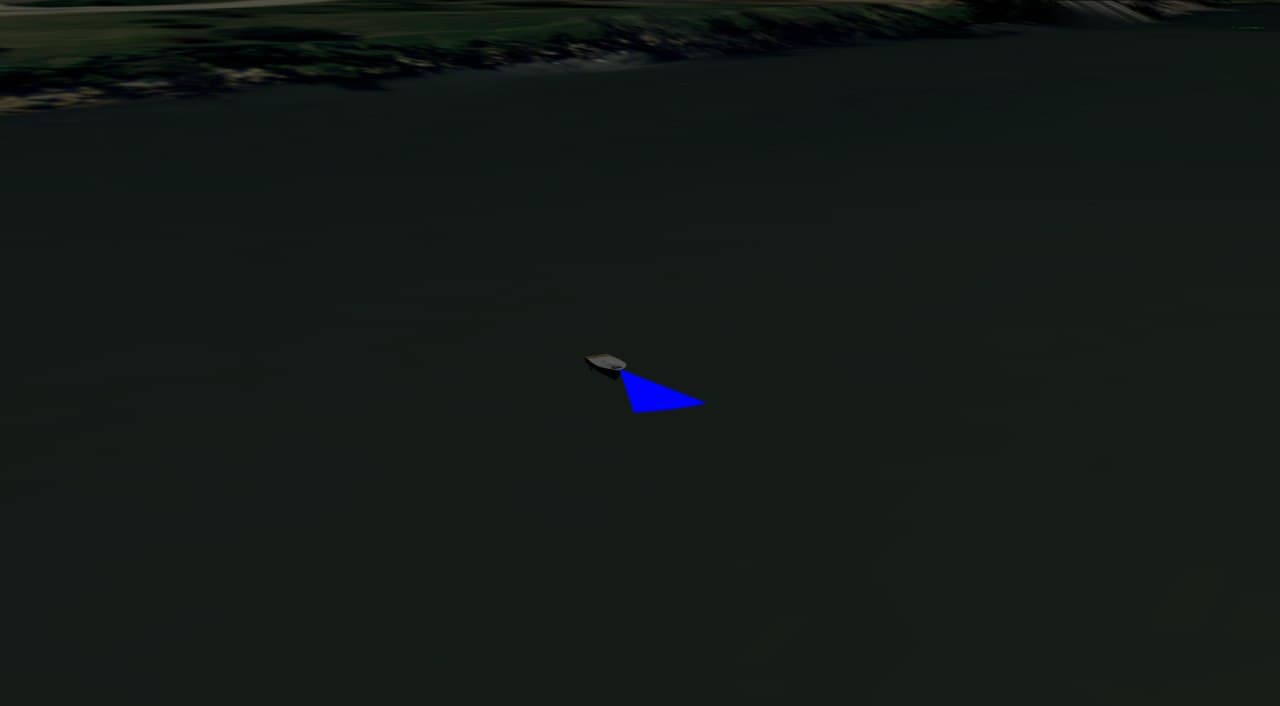
\includegraphics[width=0.8\linewidth]{sonar_boot.jpg}
	\caption{USV, Messwerte des Sonars in blau}
	\label{sonar}
\end{figure}

Die Simulationsumgebung kann man unter TODO finden und downloaden. Unser Szenario startet man mit den Befehlen:
\begin{itemize}
	\item \texttt{catkin\_make\_isolated --install}
	\item \texttt{source install\_isolated/setup.bash}
	\item \texttt{roslaunch usv\_sim rescue\_robotics\_boat\_scenario1.launch parse:=true}
	\item \texttt{roslaunch usv\_sim rescue\_robotics\_boat\_scenario1.launch parse:=false}
	\item \texttt{rosservice call /gazebo/unpause\_physics "{}"}
\end{itemize}
In dem Projekt TODO ist das implementierte Verhalten des Bootes, also das Abfahren des Gewässers mit gleichzeitiger Aufnahme der Wassertiefe, zu finden. Dieses Szenario startet man durch die Befehle:
\begin{itemize}
	\item \texttt{TODO: Bereich und Startkoordinaten angeben}
	\item \texttt{roslaunch boot usv.launch}
\end{itemize}
Die Werte TODO müssen dabei durch den gewünschten Namen der Datei, in der die Messungen gespeichert werden sollen, die GPS-Koordinaten, an denen das Boot die Messung starten soll und die Höhe und Breite des Bereichs, in dem gemessen werden soll. TODO soll durch den Abstand ersetzt werden, in dem die Messwerte gespeichert werden sollen. Nach der Simulation kann man die Ergebnissen dann in den Dateien TODO finden.
Wir haben Szenario mit verschiedenen Einstellungen gestartet:
\begin{itemize}
	\item TODO
\end{itemize}
Die Zielpunkte wurden in allen Versuchen richtig gesetzt und der Bereich damit korrekt abgefahren. Dabei wurden Orte, die sich in einem unbefahrbaren Bereich befanden, übersprungen. Unbekannte Hindernisse wurden ebenfalls immer umfahren.\\
Die Messung der Wassertiefe kann im Simulator leider nur bedingt getestet werden, da die Wasseroberfläche als Hindernis wahrgenommen wird. Deshalb werden dort momentan zufällige Messwerte generiert.

\subsection{Realität}


\section{Fazit} \label{fazit}
Unser am Anfang gestecktes Ziel, das USV durch Software zu ergänzen, die ein autonomes Befahren eines Gewässers und die gleichzeitige Aufnahme von Messwerten ermöglicht, wurde im Laufe der Projektarbeit erreicht. Auch die Simulation des Bootes ist grundsätzlich funktionsfähig. Eine Ausnahme bildet die Messung der Wassertiefe, welche bislang nicht gemessen werden kann, da der Ultraschallsensor die Wasseroberfläche als Hindernis wahrnimmt. Außerdem verfügt das Boot noch über weitere Sensoren, die wir im Modell nicht beachtet haben, da wir sie für unseren Anwendungsfall nicht benötigten. Diese sollten aber relativ unproblematisch zu unserem Modell hinzugefügt werden können, so dass unser Modell auch für weitere Projekte eine gute Grundlage bilden sollte.\\
Die Menge der Anwendungsfälle, in denen das Boot genutzt werden kann, ist bisher begrenzt. Die Messung der Wassertiefe könnte zwar dabei helfen, vermisste Personen im Wasser zu lokalisieren, aber andere Problemstellungen, wie zum Beispiel das Erkennen von Deichbrüchen und Verschmutzungen, können bis jetzt nicht abgedeckt werden. Aber auch für diese noch zu implementierenden Anwendungsfälle wird sich das bereits erreichte autonome Befahren des Gewässers sicher als nützlich herausstellen.

\bibliography{bericht}{}
\bibliographystyle{ieeetran}

\end{document}
